\documentclass[a4paper,12pt,oneside,openany,table,xcdraw]{article}
\usepackage{setspace}
\usepackage{multirow}
\usepackage{multicol}
\usepackage{hyperref}
\usepackage{caption}
\usepackage{indentfirst}

\usepackage[brazilian]{babel}
\usepackage[utf8x]{inputenc}
\usepackage{amsmath, graphicx, subfig, enumerate}
\usepackage{float, verbatim}
\usepackage[colorinlistoftodos]{todonotes}
\usepackage{makeidx}
\usepackage{geometry}

\usepackage{hhline}

\graphicspath{{../img/}}
\geometry{a4paper, hmargin={3cm, 3cm}, vmargin={3cm, 2cm} }
\setlength{\parindent}{1.0cm}
\captionsetup{font=small}

\begin{document}
\newcommand{\thedepartment}{Faculdade de Engenharia Elétrica}
\newcommand{\thecourse}{FEELT}
\newcommand{\thetitle}{AMPLIFICADOR DIFERENCIAL}
\newcommand{\thetype}{Relatório da Disciplina de Eletrônica Analógica II}
\newcommand{\theproftitle}{Bacharel em Engenharia Elétrica}
\newcommand{\thestudent}{Lesly Viviane Montúfar Berrios\\
\centering11811ETE001}
\newcommand{\theadvisor}{Prof. Gustavo Brito de Lima}
\newcommand{\thecity}{Uberlândia}

\thispagestyle{empty}\newcommand*{\themonth}{\ifthenelse{\the\month < 2}{Janeiro }
                  {\ifthenelse{\the\month < 3}{Fevereiro }
                  {\ifthenelse{\the\month < 4}{Março }
                  {\ifthenelse{\the\month < 5}{Abril }
                  {\ifthenelse{\the\month < 6}{Maio }
                  {\ifthenelse{\the\month < 7}{Junho }
                  {\ifthenelse{\the\month < 8}{Julho }
                  {\ifthenelse{\the\month < 9}{Agosto }
                  {\ifthenelse{\the\month < 10}{Setembro }
                  {\ifthenelse{\the\month < 11}{Outubro }
                  {\ifthenelse{\the\month < 12}{Novembro }{Dezembro }}}}}}}}}}}}
                  
\begin{titlepage}
\begin{center}

	\vspace{-0.5cm}

  \begin{figure}[hbt!]
		\begin{center}
		   
\includegraphics[width=2.8cm]{ufu-logo.png}
		\end{center}
	\end{figure}
 	%\vspace{-4cm}

%\begin{doublespacing}

  \Large{\textbf{Universidade Federal de Uberlândia}}\\
  \large{\thedepartment}\\
  \large{\thecourse}\\


\vspace{5.8cm}
  \par
  \large\textbf{\thetitle}
\vspace{5.8cm} 

%\end{doublespacing}
  \par
  \thetype\\
  por\\
  %\hspace{2cm}\large{}\\

\vspace{0.8cm}
\par
  \normalsize{\thestudent}\\ [2cm]
  \theadvisor

\par\vfill
  \thecity, \themonth / \the\year

\end{center}

\end{titlepage}

%% Comeca o documento !

\onehalfspacing
\tableofcontents 
\newpage

 %%%%%%%%%%%%%%%%%%%%%%%%%%%%%%%%%%%%%%%%%%%%%%%%%%%%%%%%%%%%%%%%%%%%%%%%%%%%
\section{Objetivos} % 2,5 %
Realizar a análise em corrente contínua (CC) e alternada (CA) de um circuito amplificador diferencial, com intuito de confirmar experimentalmente o procedimento teórico.

 %%%%%%%%%%%%%%%%%%%%%%%%%%%%%%%%%%%%%%%%%%%%%%%%%%%%%%%%%%%%%%%%%%%%%%%%%%%%
\section{Introdução teórica} 
%qu'Est-ce que c'est? Histoire


% À quoi ça sert? Applications
O amplificador diferencial é o estágio de entrada da maioria dos amplificadores operacionais, daí a importância de estudá-lo. Além disso, tem a função de aumentar a impedância de entrada, reduzir a corrente de polarização e o \emph{offset} da tensão de saída. A Figura \ref{intro:amp-dif} exemplifica a estrutura de um amplificador diferencial.

\vspace{0.2cm}
\begin{figure}[H]
\centering
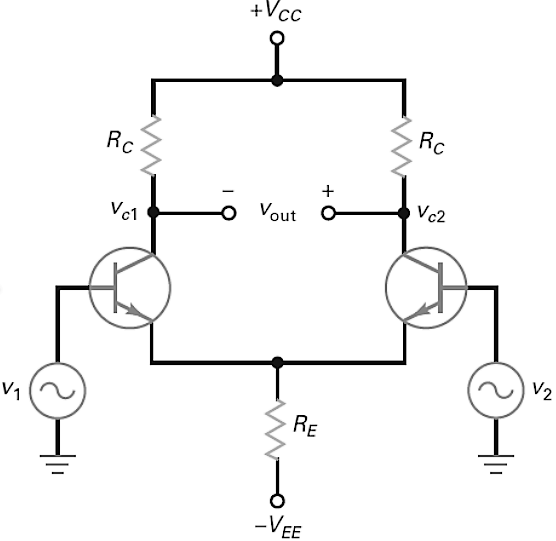
\includegraphics[width=12cm]{amp-dif}
\caption{Amplificador diferencial.}
\label{intro:amp-dif}
\end{figure}
\vspace{0.3cm}

Nesse circuito, a relação entre entrada e saída é dada como na Equação \ref{vout}, e, da análise em corrente contínua (CC), percebe-se que o \emph{offset} de tensão de saída é nulo quando as tensões de entrada estão em fase e são de mesma amplitude.

\begin{equation} \label{vout}
V_{out} = A_v\ (V_{in} ^+ - V_{in} ^-)
\end{equation}


 %%%%%%%%%%%%%%%%%%%%%%%%%%%%%%%%%%%%%%%%%%%%%%%%%%%%%%%%%%%%%%%%%%%%%%%%%%%%
\section{Procedimento Experimental}
\subsection{Materiais e ferramentas} % 2,5%

\singlespacing
\begin{itemize}
\begin{multicols}{2}
\item \emph{2 transistores BC337 ou similar;}
\item \emph{2 resistores 6k8;}
\item \emph{1 resistor 5k6;}
\item \emph{1 resistor de 1k;}
\item \emph{1 resistor de 100k;}\columnbreak

\item \emph{1 Fonte de alimentação simétrica;}
\item \emph{1 Multímetro;}
\item \emph{1 Gerador de Funções;}
\item \emph{1 Osciloscópio}
\end{multicols}

\end{itemize}
\onehalfspacing

\vspace{0.2cm}
\subsection{Montagem} % 2,5%
A montagem a ser utilizada no experimento trata-se do amplificador diferencial da Figura \ref{proc:montagem}. Assim, da análise a nível CC tem-se o circuito da Figura \ref{proc:CC}, enquanto que para o nível CA, o da Figura \ref{proc:CA}. Cada circuito da Figura \ref{proc:analise}, será análisado e montado separadamente durante o experimento, para assim poder coletar os dados de $V_{out, 1}$, $V_{out, 2}$ e $I_{T}$.

\vspace{0.3cm}
\begin{figure}[H]
\centering
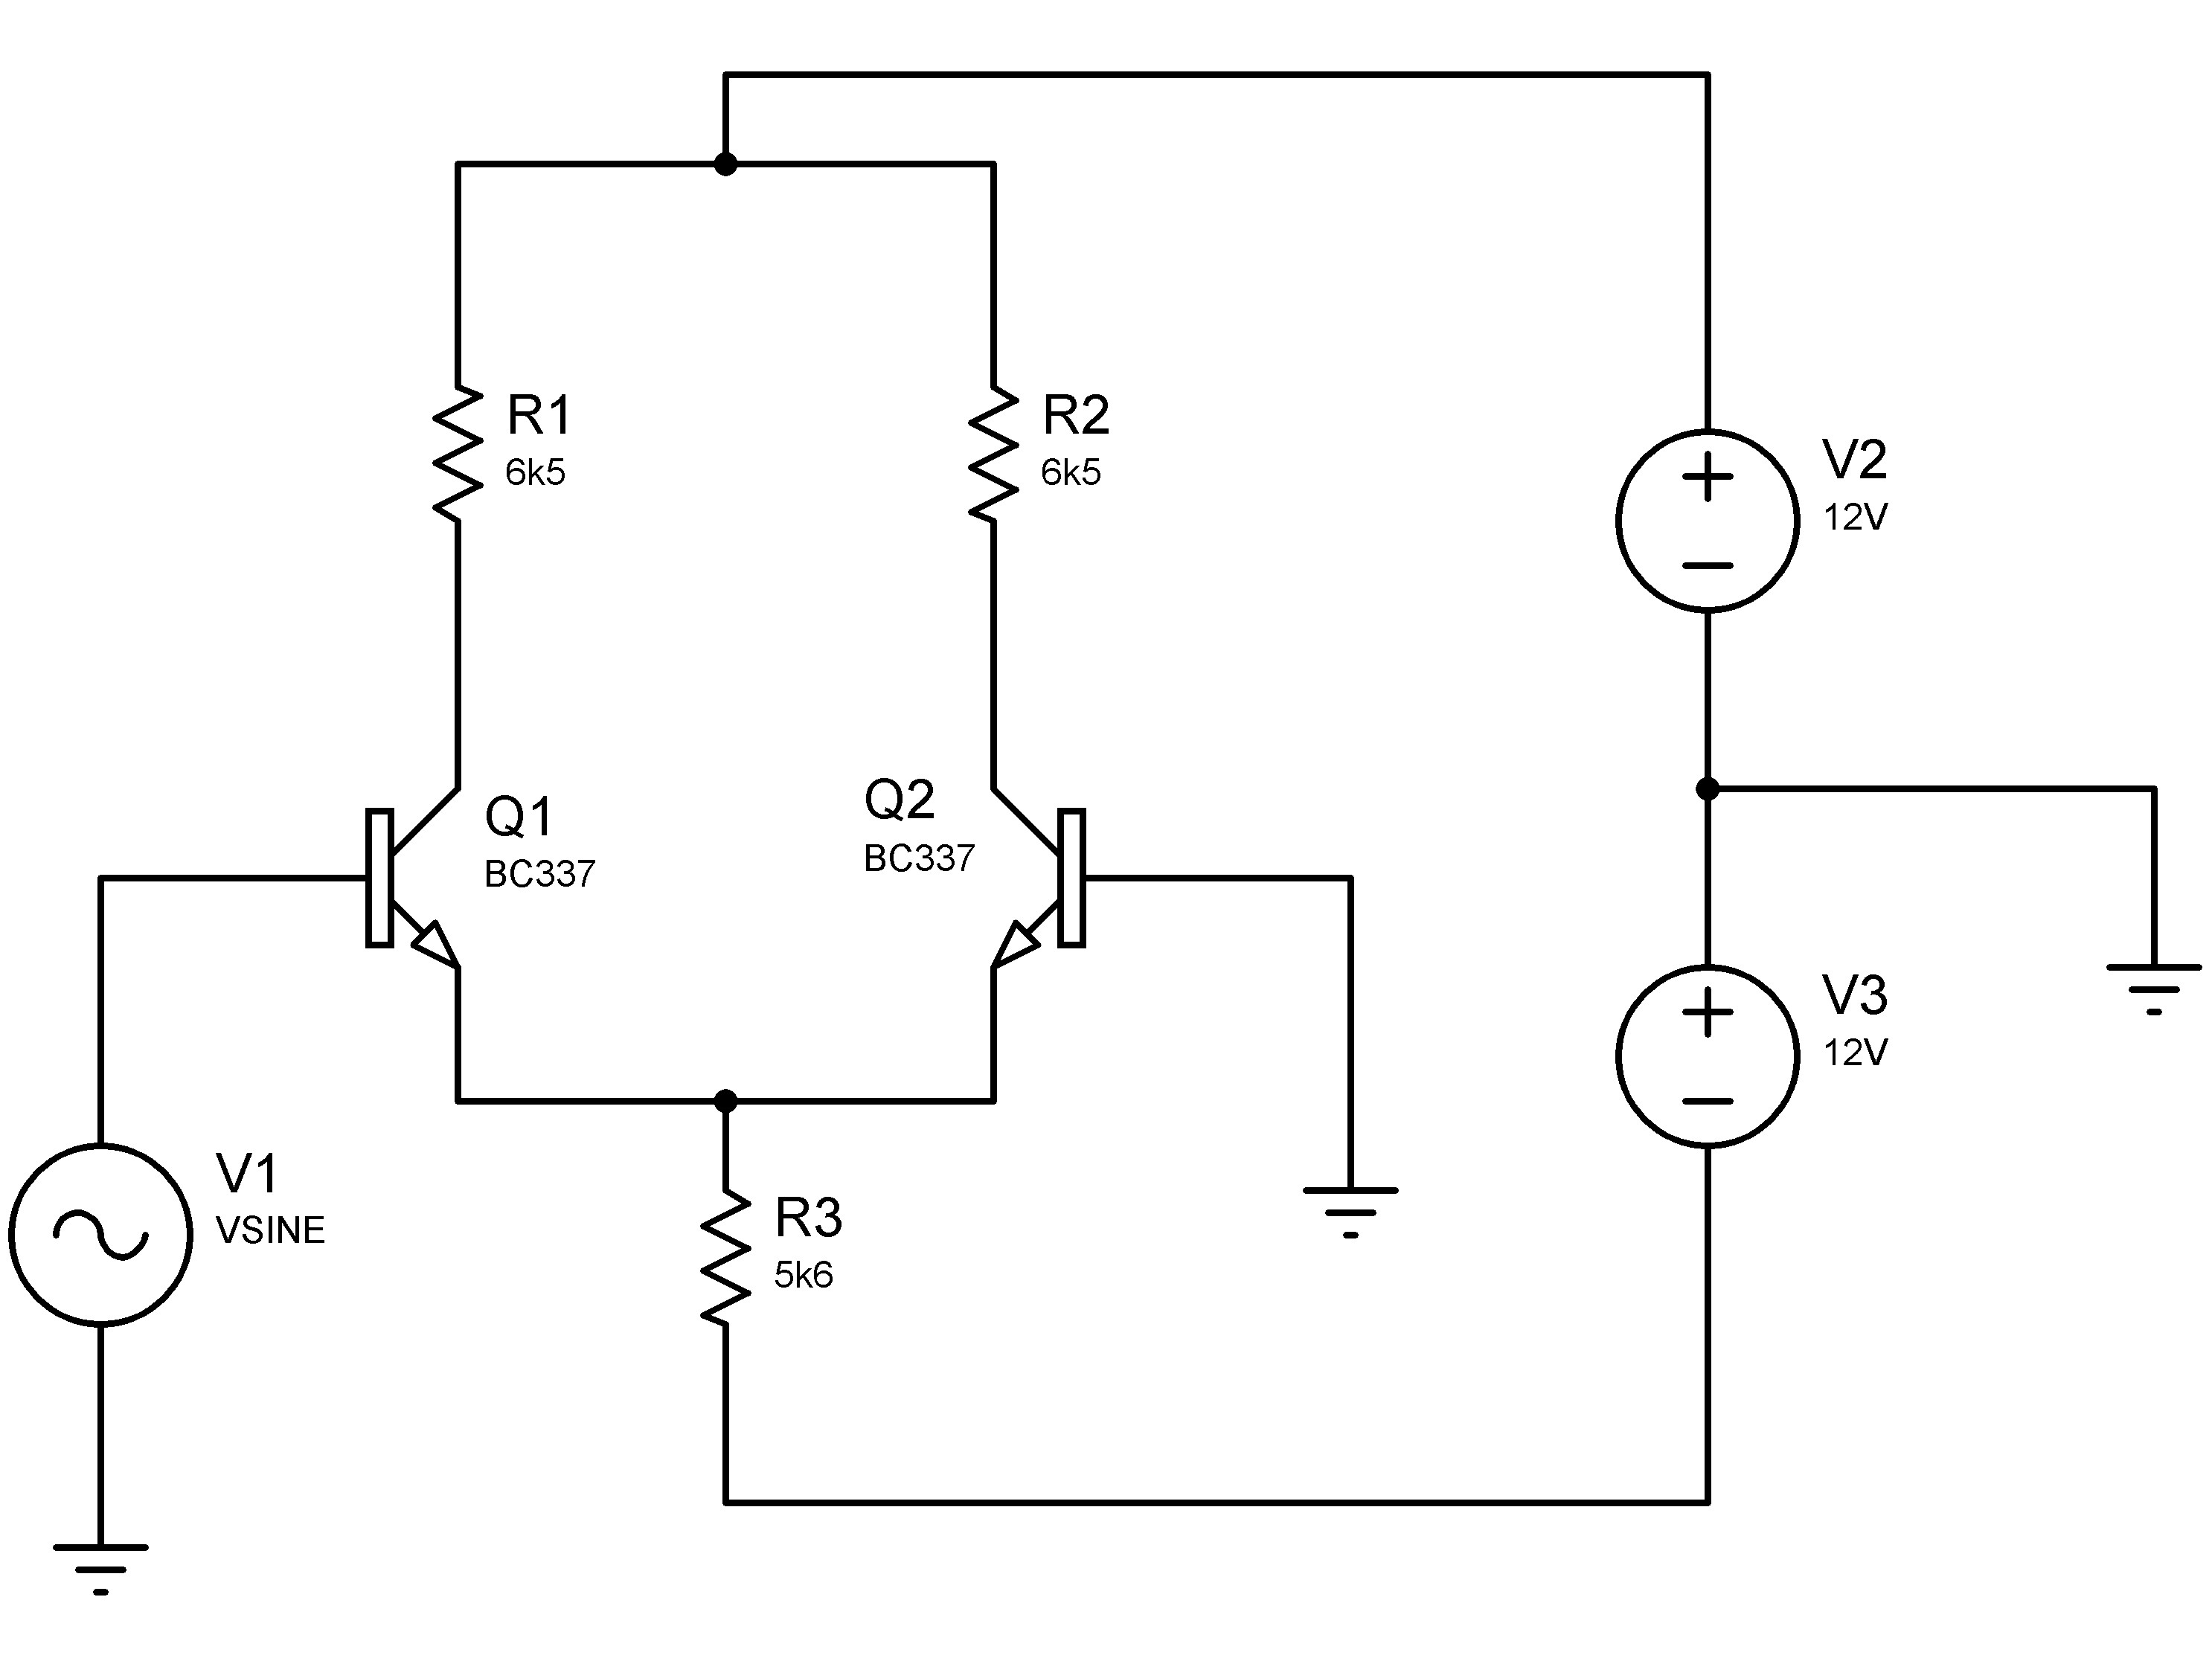
\includegraphics[width=13cm]{montagem}
\caption{Montagem do amplificador diferencial.}
\label{proc:montagem}
\end{figure}
\vspace{0.5cm}

\begin{figure}[H]
\center
\subfloat[][]{\label{proc:CC}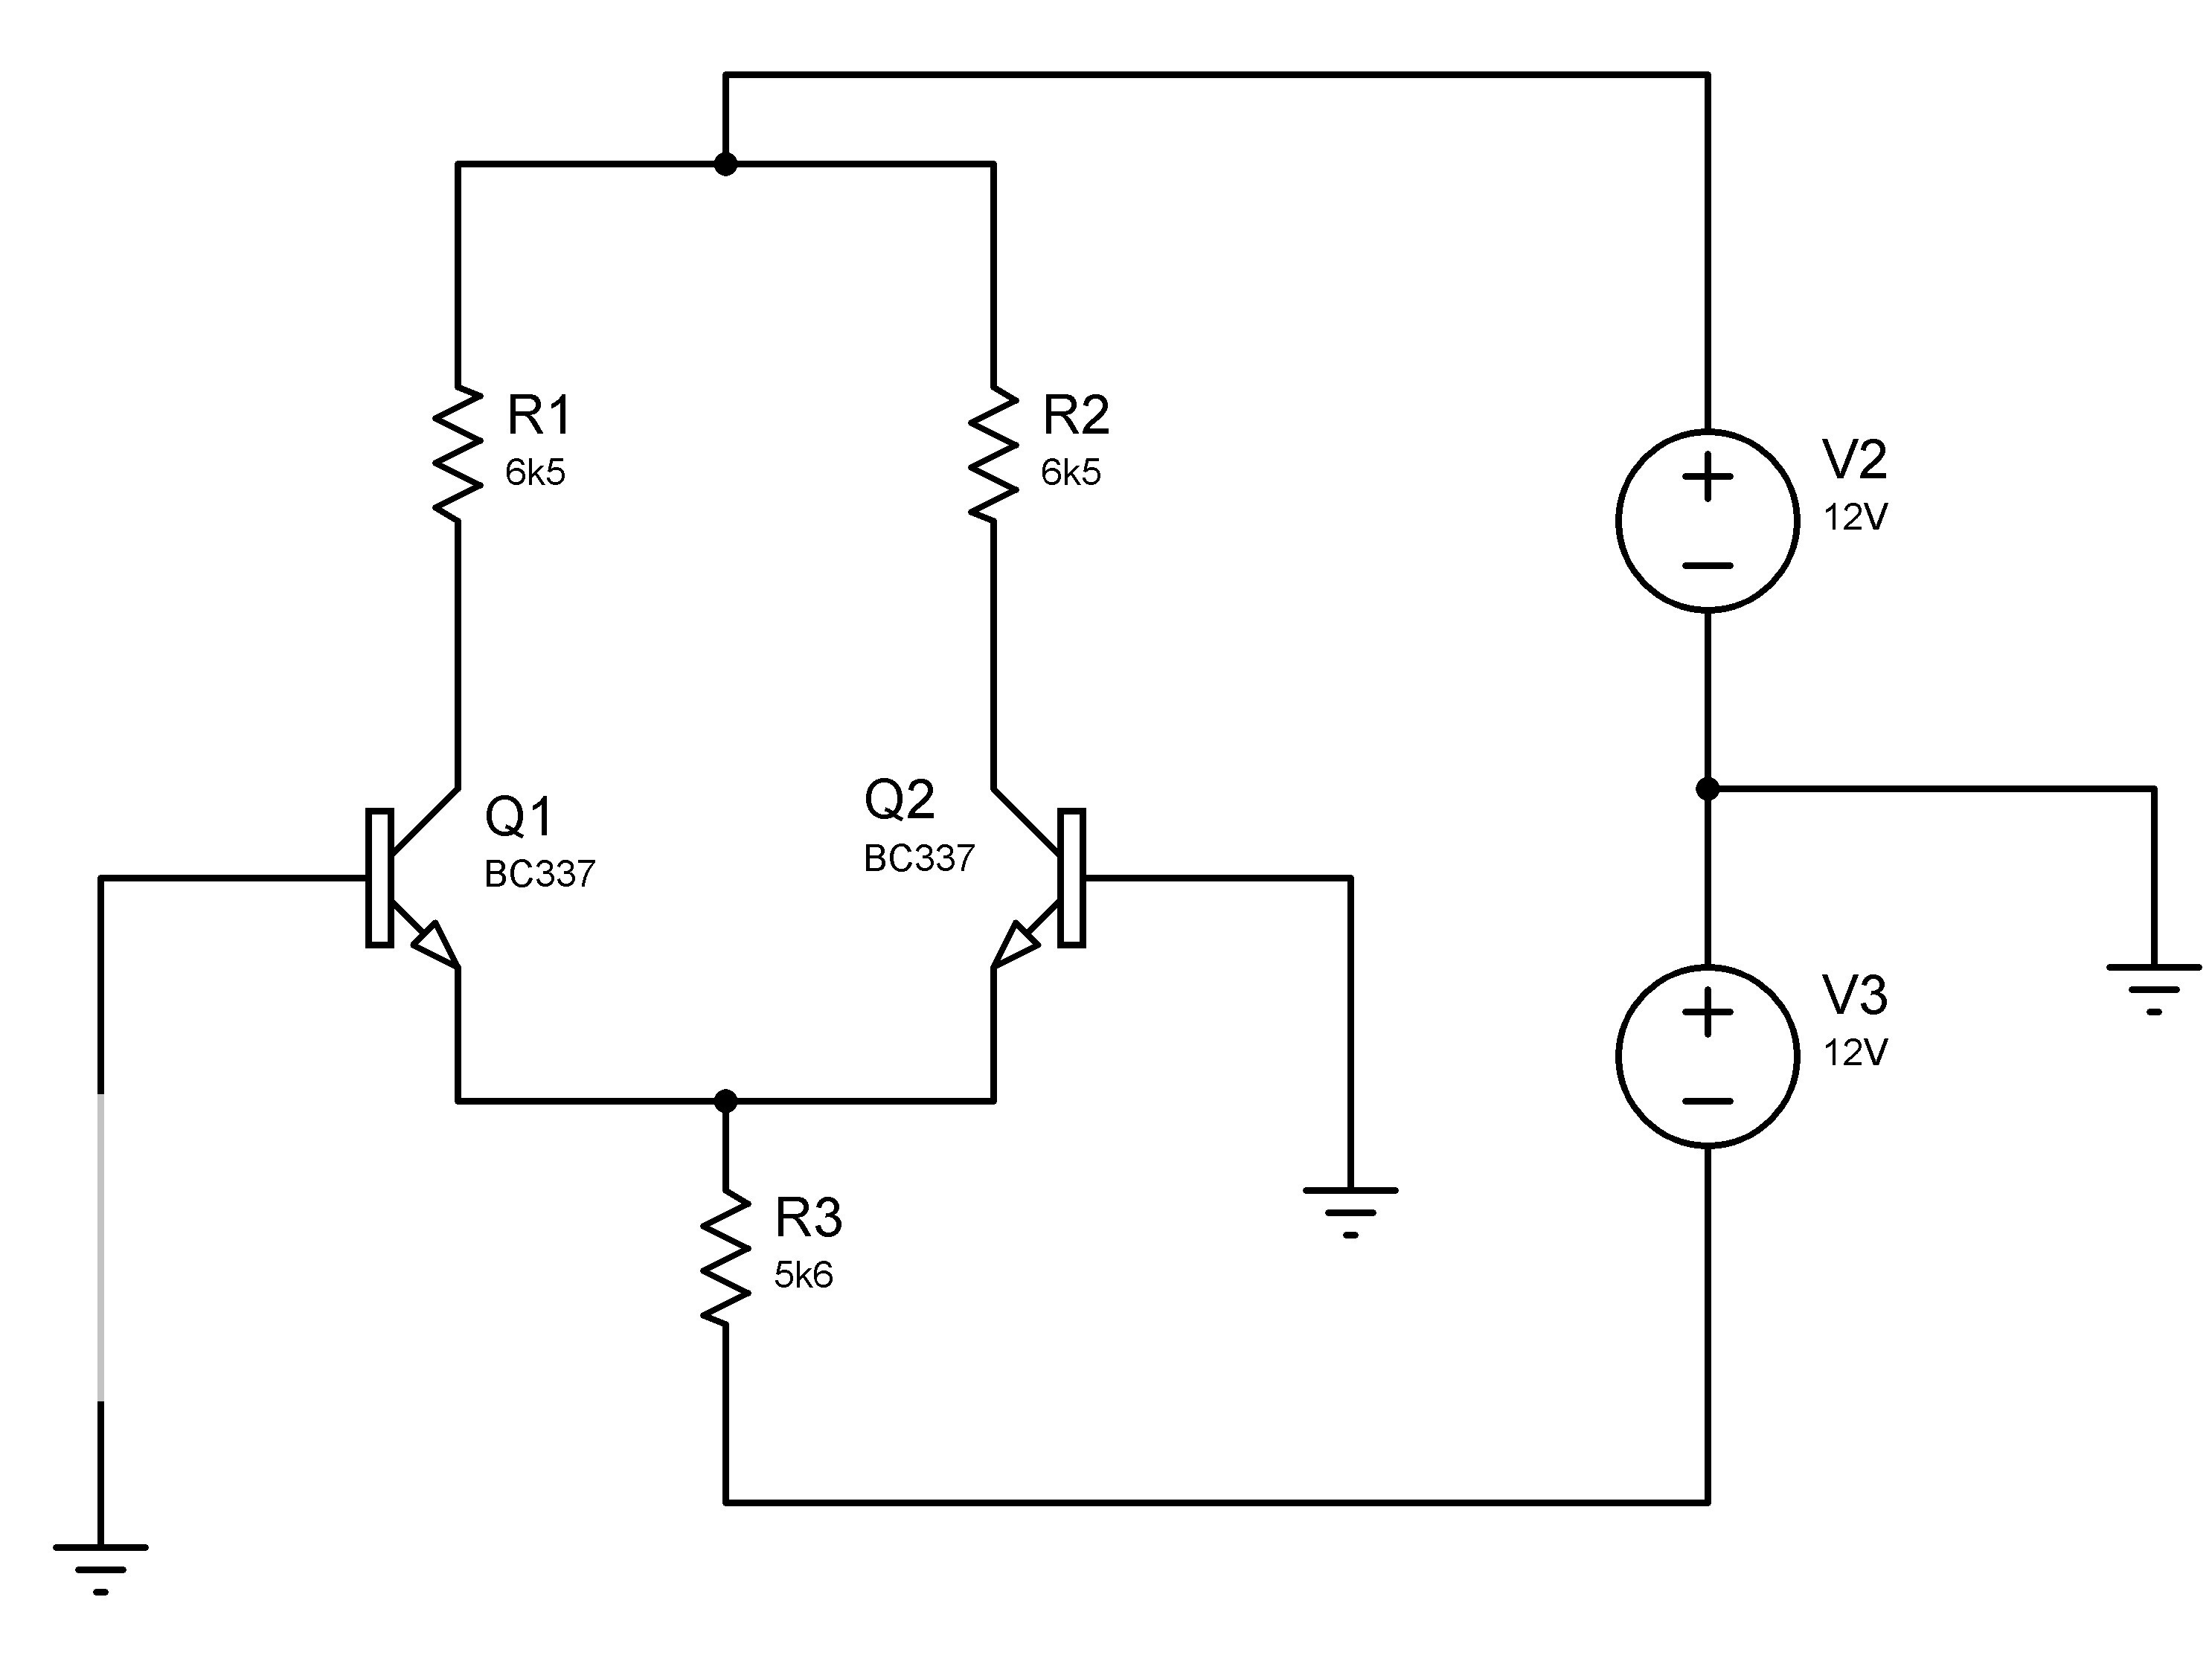
\includegraphics[height=5cm]{CC}}\hfill
\subfloat[][]{\label{proc:CA}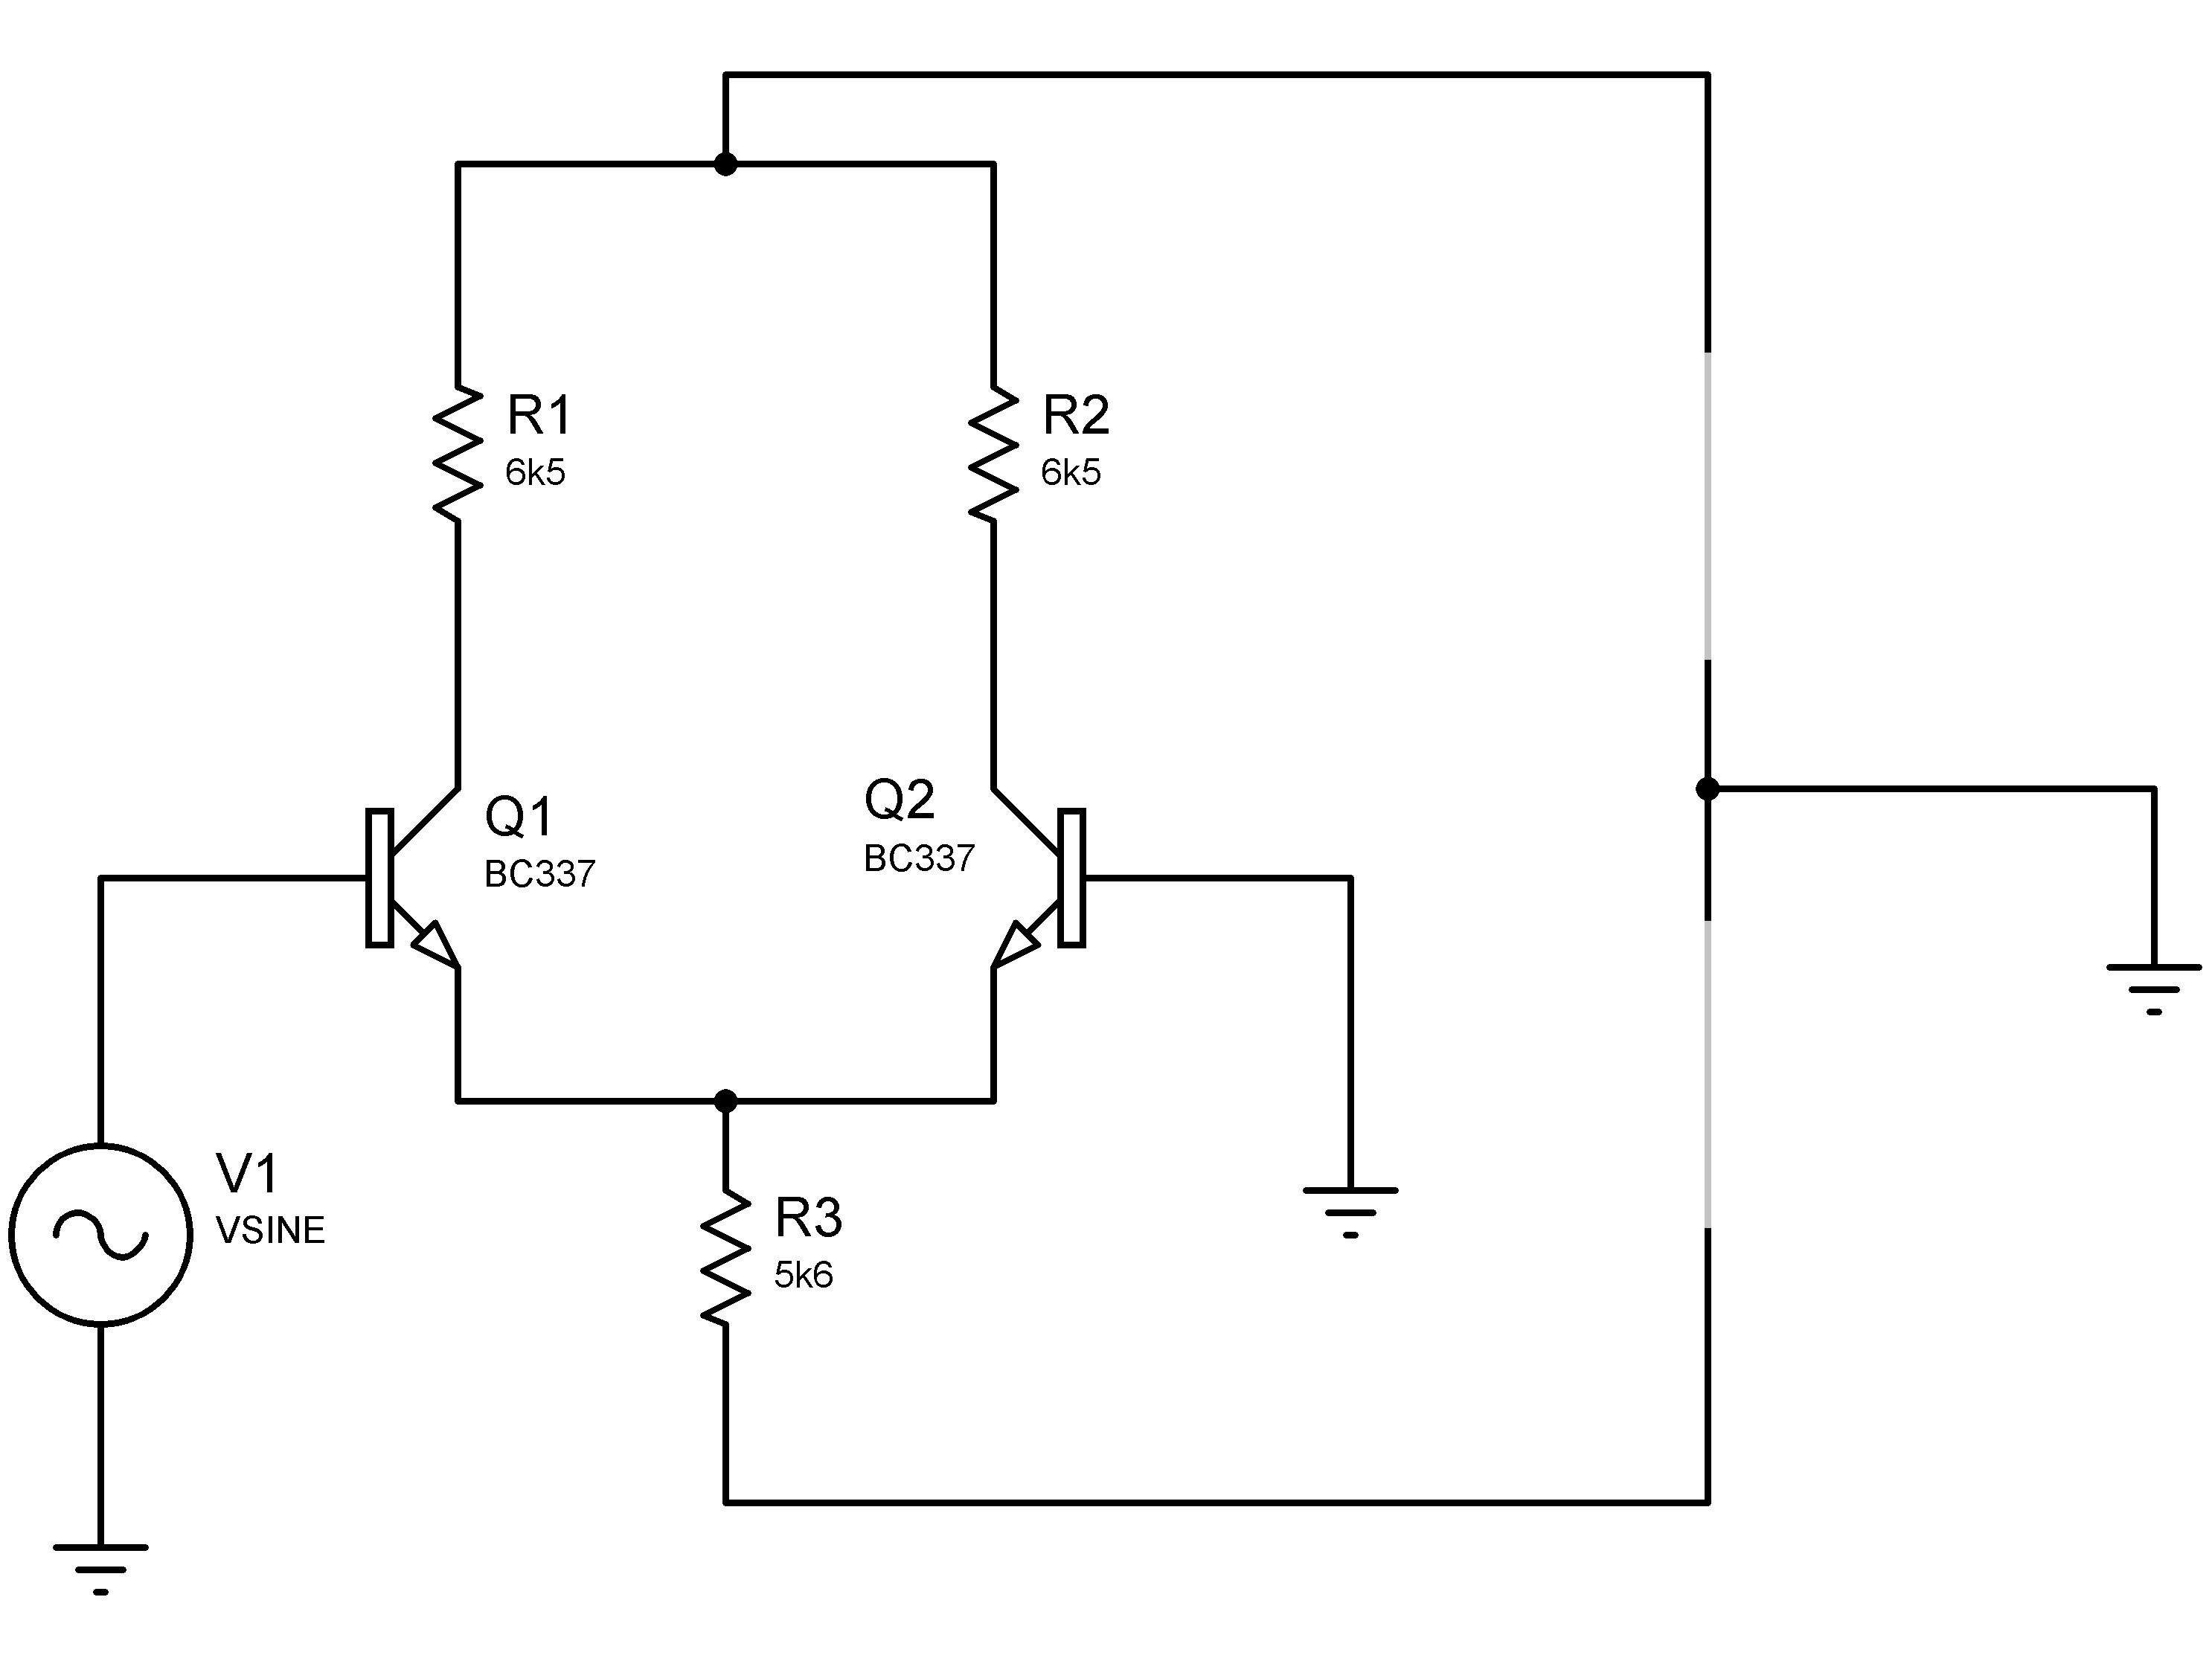
\includegraphics[height=5cm]{CA}}
\caption{Análise (a) CC e (b) CA do circuito amplificador diferencial.}
\label{proc:analise}
\end{figure}
\vspace{0.5cm}

\section{Dados teóricos e experimentais}
Durante o experimento, a partir da análise CC, utilizando-se o circuito da Figura \ref{proc:CC}, obteve-se os dados experimentais da Tabela \ref{dados}, os quais podem ser determinados teoricamente por meio das Equações \ref{eq:IT}, \ref{eq:Vout1} e \ref{eq:Vout2}. Considere que $I_{C} =I_{E} =  \dfrac{I_{T}}{2}$, $V_{BE} = 0,7 V$ e $V_{CC}=12 V$.
\vspace{0.2cm}

\begin{equation} \label{eq:IT}
I_{T} = \dfrac{-V_{BE} + V_{CC}}{R_{3}}
\end{equation}

\begin{equation} \label{eq:Vout1}
V_{out,1} = V_{CC} - (\dfrac{I_{T}}{2})\ R_{1}
\end{equation}


\begin{equation} \label{eq:Vout2}
V_{out,2} = V_{CC} - (\dfrac{I_{T}}{2})\ R_{2}
\end{equation}
 
\vspace{0.3cm}
\begin{table} [H]
\centering
\def\arraystretch{1.38}
\caption{Tensões de polarização do amplificador diferencial. } \label{dados}
\begin{tabular}{|c|c|c|c|} 
\hhline{~---|}
\multicolumn{1}{c|}{}                            & {\cellcolor[rgb]{0.937,0.937,0.937}}\textbf{$I_{T}$(mA)} & {\cellcolor[rgb]{0.937,0.937,0.937}}\textbf{$V_{out, 1}$ (V)} & {\cellcolor[rgb]{0.937,0.937,0.937}}\textbf{$V_{out, 2}$~(V)}  \\ 
\hline
{\cellcolor[rgb]{0.937,0.937,0.937}}Teórico      & 2,0179                                                   & 5,4420                                                        & 5,4452                                                         \\ 
\hline
{\cellcolor[rgb]{0.937,0.937,0.937}}Experimental &                                                          &                                                               &                                                                \\ 
\hline
{\cellcolor[rgb]{0.937,0.937,0.937}}Erro (\%)        &                                                          &                                                               &                                                                \\
\hline
\end{tabular}
\end{table}

\vspace{0.3cm}
Já a Figura \ref{proc:CA} permite realizar a análise CA. Substitui-se o transistor pelo modelo equivalente $T$ ou $\pi$ e assim tem-se as relações das Equações \ref{saidasimples} e \ref{saidadif}, que correspondem ao ganho no caso de saídas simples e diferencial respectivamente. Considere a tensão térmica $V_{T}=25 mV$ e a resistência equivalente no terminal emissor $r'_{E}=\dfrac{V_{T}}{I_{E}} = 24,7795 \Omega$, já que $I_{E} = \dfrac{I_{T}}{2} = 1,0089 A$. A Tabela \ref{ganho} contemplam a comparação entre os dados teóricos e experimentais obtidos.

\vspace{0.2cm}
\begin{equation} \label{saidasimples}
A_{simples} = \dfrac{V_{T}}{2 r'_{E}}
\end{equation}

\begin{equation} \label{saidadif}
A_{diferencial} = \dfrac{V_{T}}{r'_{E}}
\end{equation}

\vspace{0.3cm}
\begin{table} [H]
\centering
\def\arraystretch{1.38}
\caption{Ganho no caso de saída simples e diferencial, respectivamente.} \label{ganho}
\begin{tabular}{|c|c|c|} 
\hhline{~--|}
\multicolumn{1}{c|}{}                            & {\cellcolor[rgb]{0.937,0.937,0.937}}\begin{tabular}[c]{@{}>{\cellcolor[rgb]{0.937,0.937,0.937}}c@{}}\textbf{Ganho em}\\\textbf{Saída Simples}\end{tabular} & {\cellcolor[rgb]{0.937,0.937,0.937}}\begin{tabular}[c]{@{}>{\cellcolor[rgb]{0.937,0.937,0.937}}c@{}}\textbf{Ganho em}\\\textbf{Saída Diferencial}\end{tabular}  \\ 
\hline
{\cellcolor[rgb]{0.937,0.937,0.937}}Teórico      & 131,157                                                                                                                                                             & 262,314                                                                                                                                                                  \\ 
\hline
{\cellcolor[rgb]{0.937,0.937,0.937}}Experimental &                                                                                                                                                                     &                                                                                                                                                                          \\ 
\hline
{\cellcolor[rgb]{0.937,0.937,0.937}}Erro (\%)    &                                                                                                                                                                     &                                                                                                                                                                          \\
\hline
\end{tabular}
\end{table}

 %%%%%%%%%%%%%%%%%%%%%%%%%%%%%%%%%%%%%%%%%%%%%%%%%%%%%%%%%%%%%%%%%%%%%%%%%%%%
\newpage
\section{Simulação} 
Da simulação computacional, pode-se confirmar os valores das grandezas teóricas. Utilizando-se o software \emph{PROTEUS}, a simulação do esquemático da Figura \ref{sim:circuito} fornece os dados dispostos na Tabela \ref{sim:dados}. 
Ademais, a simulação permitiu recolher dados analógicos, no intervalo de tempo de [0, 1ms], das saídas $V_{out, 1}$ e $V_{out, 2}$, $V_{out, 2}-V_{out, 1}$ e da corrente $I_{T}$, contemplados nas Figuras \ref{sim:out1}, \ref{sim:out2}, \ref{sim:2-1} e \ref{sim:IT}.

\vspace{0.5cm}
\begin{figure}[H]
\centering
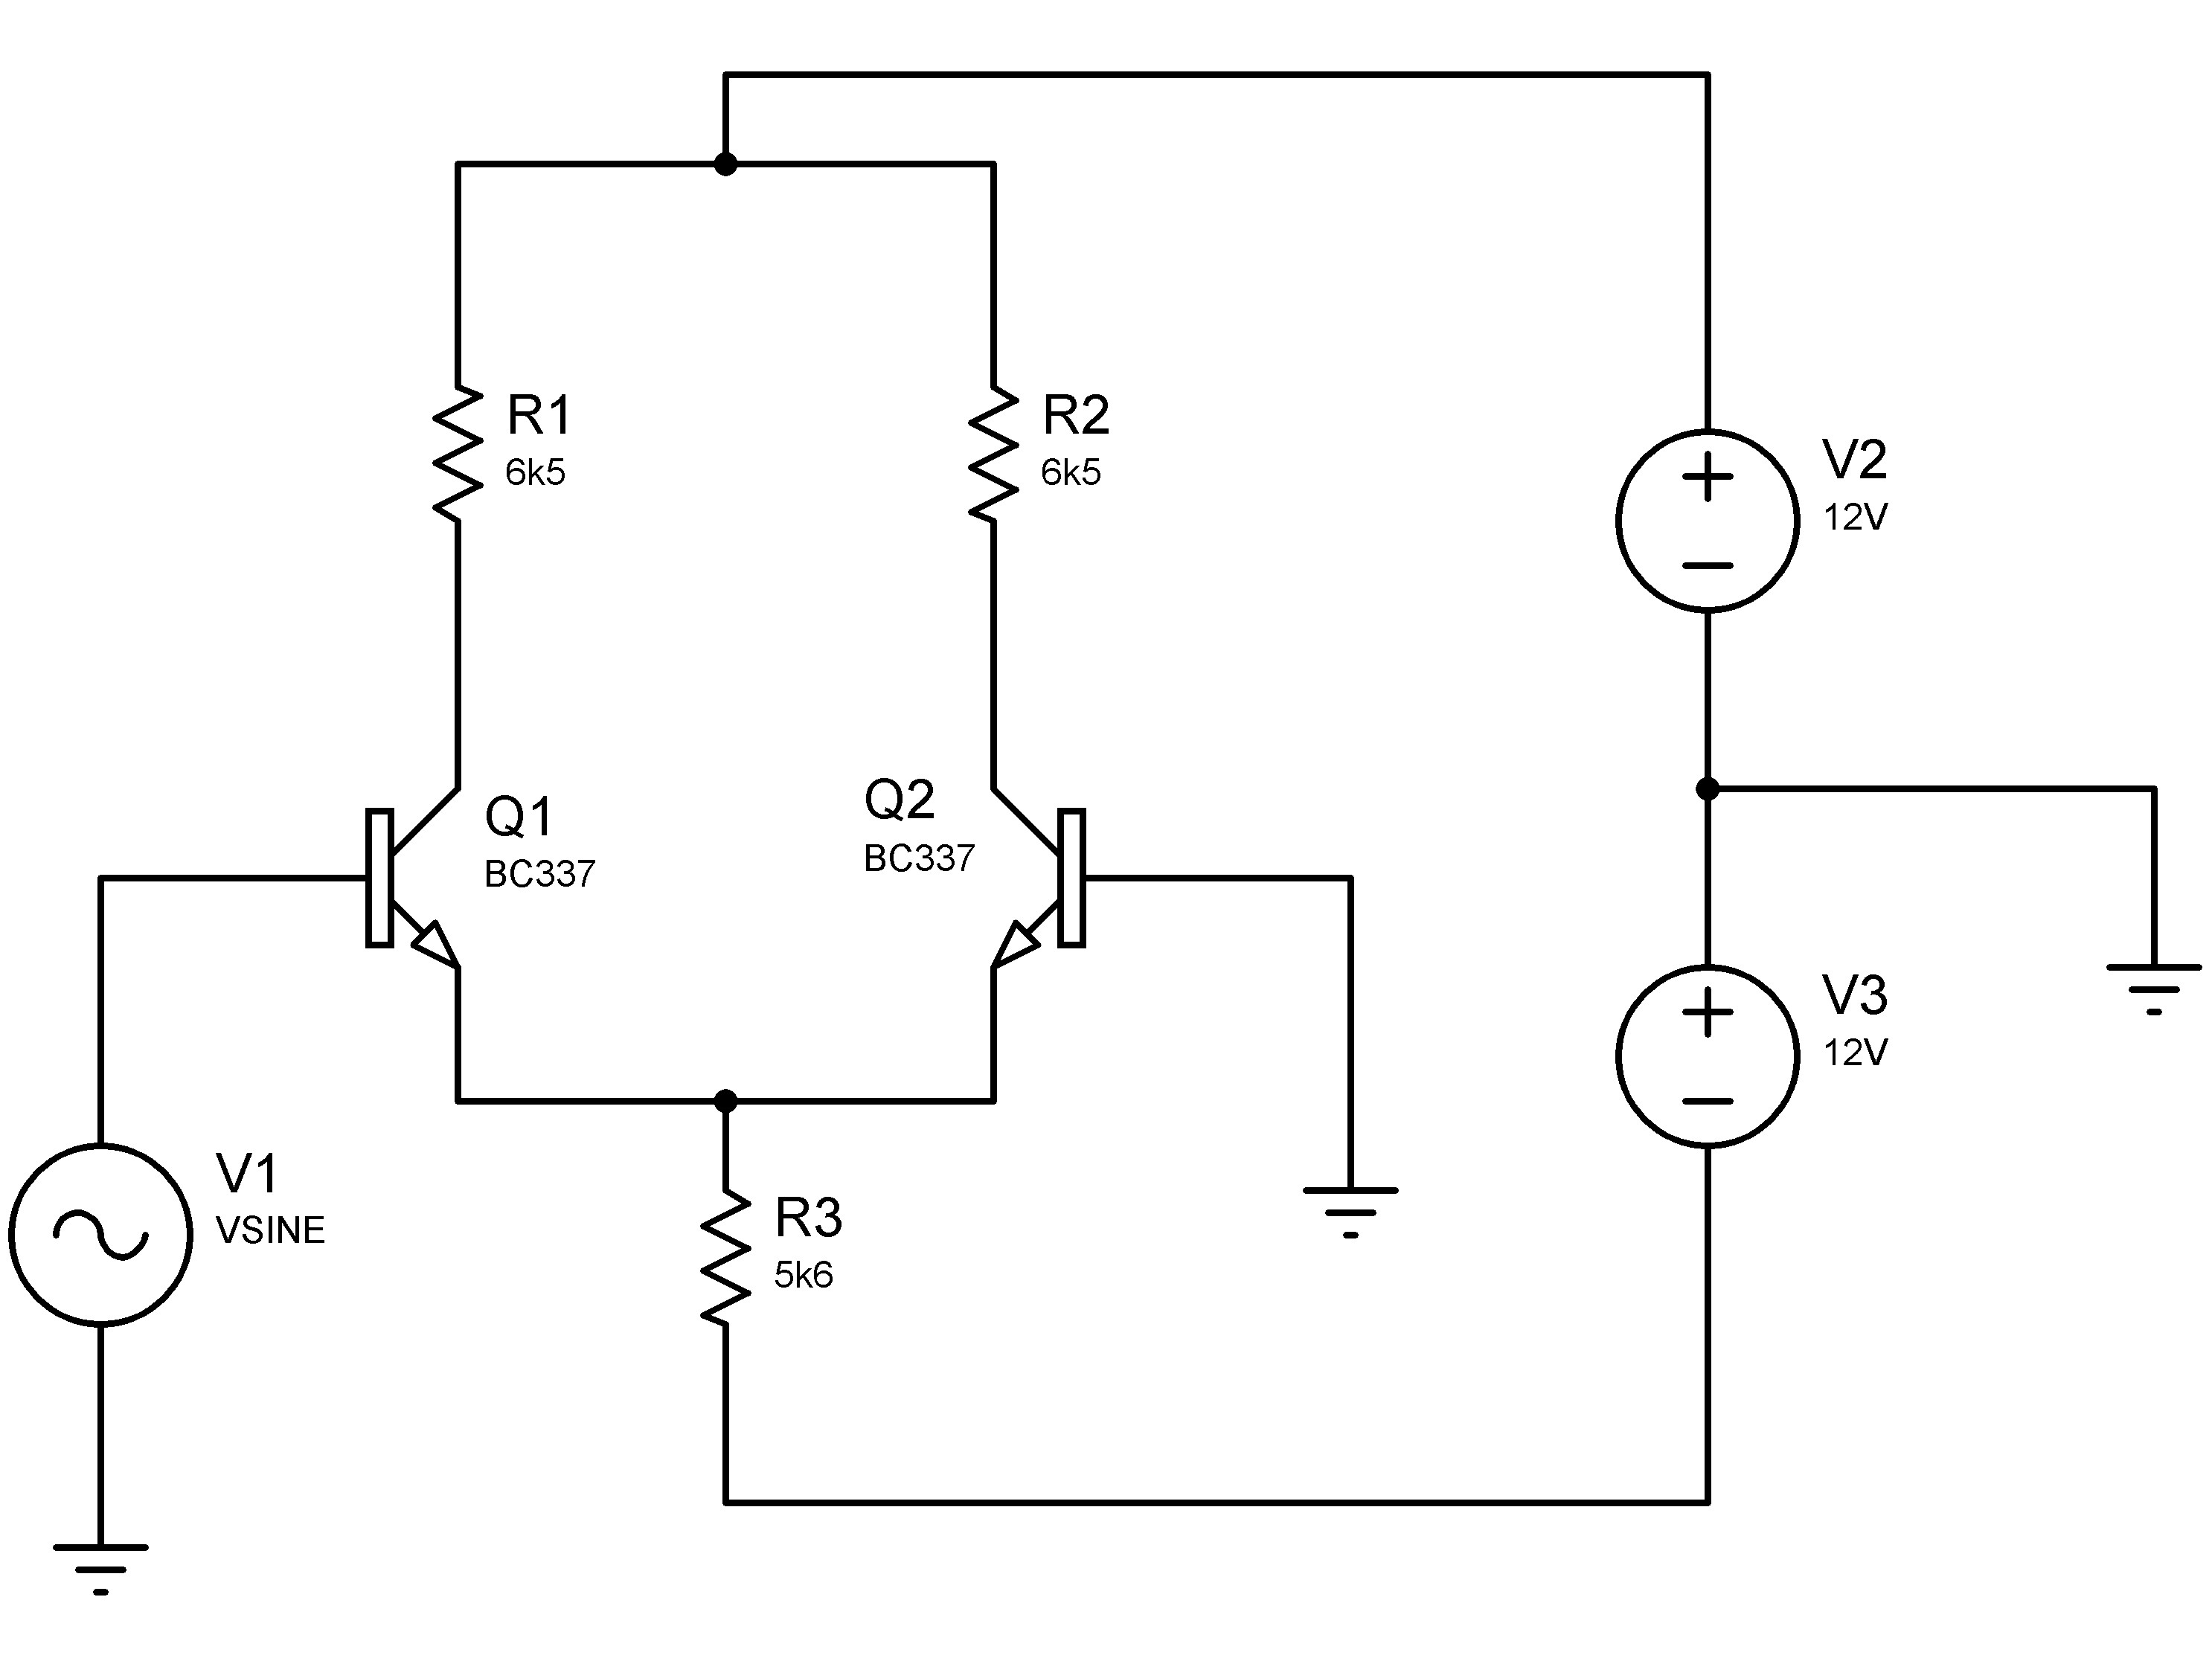
\includegraphics[width=13cm]{sim-circuito}
\caption{Circuito esquemático.}
\label{sim:circuito}
\end{figure}

\begin{figure}[H]
\center
\subfloat[]{\label{sim:out1}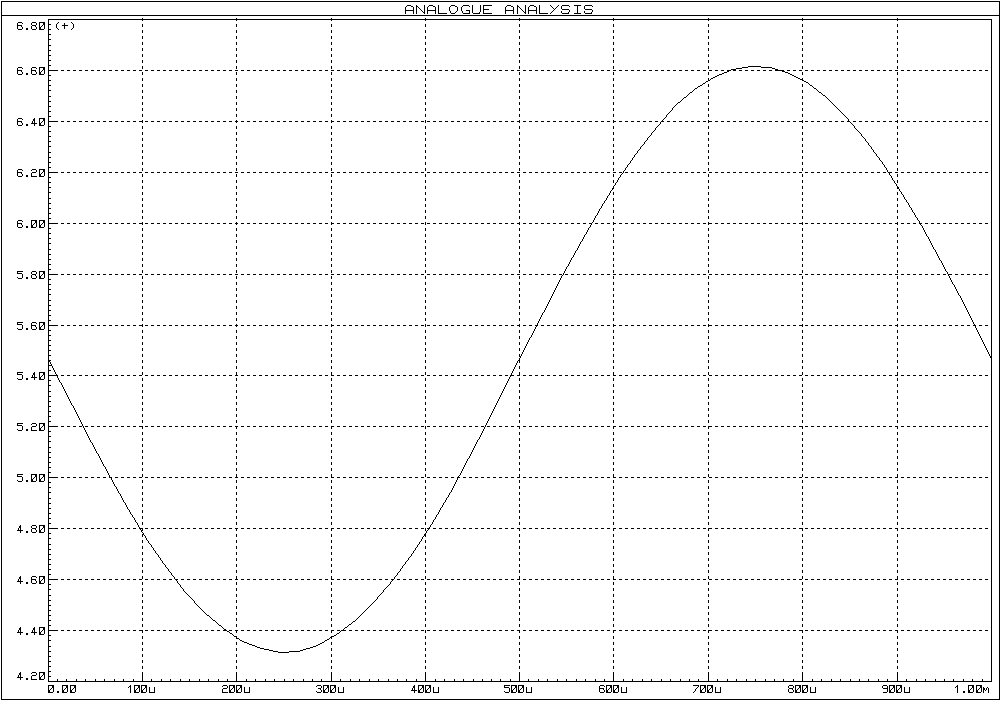
\includegraphics[height=5cm]{analog-wave1}}\hfill
\subfloat[]{\label{sim:out2}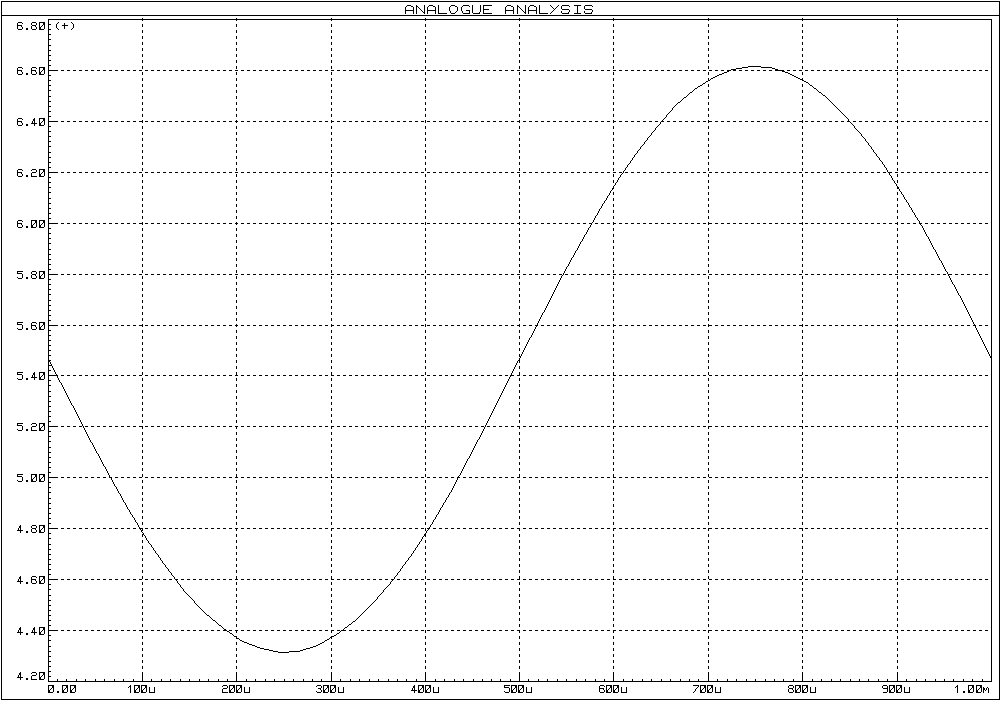
\includegraphics[height=5cm]{analog-wave2}} 
\caption{Dados analógicos das saídas (a) $V_{out,1}$ e (b) $V_{out,2}$.}
\label{sim:out}
\end{figure}
\vspace{0.5cm}

\begin{figure}[H]
\center
\subfloat[]{\label{sim:2-1}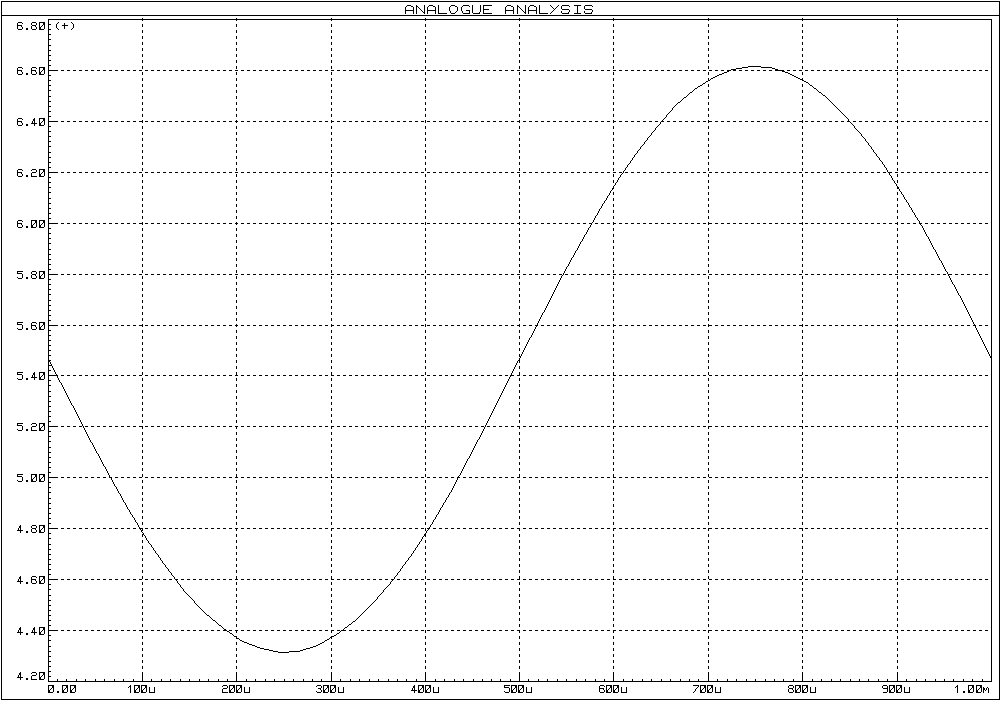
\includegraphics[height=5cm]{analog-dif}}\hfill
\subfloat[]{\label{sim:IT}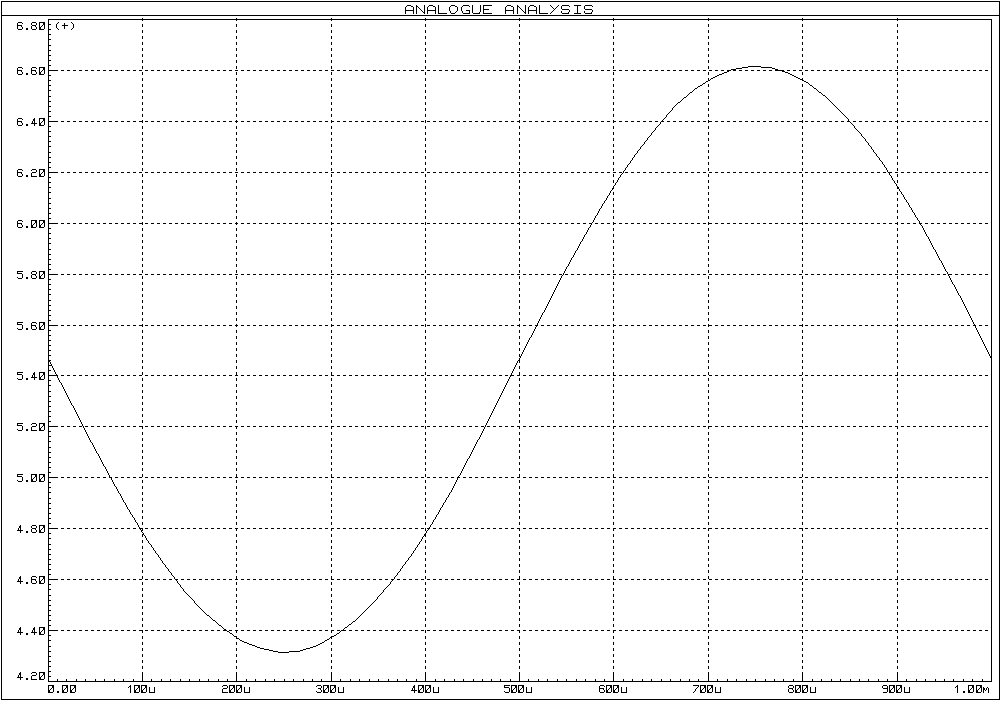
\includegraphics[height=5cm]{analog-IT}}
\caption{Dados analógicos da (a) saída diferencial $V_{out,1} - V_{out,2}$ e (b) corrente $I_{T}$.}
\label{sim:conclusoes}
\end{figure}

\vspace{0.3cm}
\begin{table} [H]
\centering
\def\arraystretch{1.38}
\caption{Tensões de polarização do amplificador diferencial obtidos na simulação.} \label{sim:dados}
\label{dados}
\begin{tabular}{|c|c|c|c|} 
\hhline{~---|}
\multicolumn{1}{c|}{}                         & {\cellcolor[rgb]{0.937,0.937,0.937}}\textbf{$I_{T}$(mA)}  & {\cellcolor[rgb]{0.937,0.937,0.937}}\textbf{$V_{out, 1}$ (V)}  & {\cellcolor[rgb]{0.937,0.937,0.937}}\textbf{$V_{out, 2}$\textasciitilde{}(V)}   \\ 
\hline
{\cellcolor[rgb]{0.937,0.937,0.937}}Teórico   & 2,0179                                                    & 5,4420                                                         & 5,4452                                                                          \\ 
\hline
{\cellcolor[rgb]{0.937,0.937,0.937}}Simulação &                                                           &                                                                &                                                                                 \\ 
\hline
{\cellcolor[rgb]{0.937,0.937,0.937}}Erro (\%) &                                                           &                                                                &                                                                                 \\
\hline
\end{tabular}
\end{table}

 %%%%%%%%%%%%%%%%%%%%%%%%%%%%%%%%%%%%%%%%%%%%%%%%%%%%%%%%%%%%%%%%%%%%%%%%%%%%
\section{Resultados e Discusões} 

\subsection{Análise comparativa}
No decorrer do relatório, tem-se a comparação entre os dados teóricos, experimentais e de simulação, dos quais não se espera grande diferença, à exceção dos experimentais, que podem sofrer alteração de condições devido ao meio - que gera incerteza na medida.

\subsection{Saída simples vs. saída diferencial}
A escolha pela saída simples ou diferencial depende da aplicação. Como analisado teoricamente e experimentalmente, a saída diferencial oferece um nível de \emph{offset} quase nulo, conforme a Figura \ref{sim:2-1}, além do dobro de ganho comparando quando o amplificador é usado em saída simples, pela Tabela \ref{ganho}. Essas características permitem que seja aplicado, por exemplo, em ... .

Enquanto que quando usado em saída simples, pode ser aplicado em diversas outras aplicações em que ... é essencial. Por exemplo, a ... utiliza esse aspectos com o intuito de ... . 

 %%%%%%%%%%%%%%%%%%%%%%%%%%%%%%%%%%%%%%%%%%%%%%%%%%%%%%%%%%%%%%%%%%%%%%%%%%%%
\section{Conclusões} 

\newpage
\begin{thebibliography}{9} 
% Introdução
\bibitem{sedra}
    Sedra, A.; Simth, K; 
    “Análise de Circuitos Em Engenharia”, Oxford University Press, $5^a$ Ed., 2004.

\bibitem{malvino}
    Malvino; 
    “Eletrônica”, Pearson, $5^a$ Ed., 2004.

\bibitem{boylestad}
    Boylestad, R;
    “Intrdução À Análise de Circuitos”, Pearson, $10^a$ Ed., 2004.

\end{thebibliography}
\end{document}
